\chapter{Implementação}

Neste capítulo descrevemos brevemente o sistema, abordando a organização de seus arquivos componentes e a estratégia de organização do software tendo em vista a criação de uma estrutura de fácil manutenção e expansão.

\section{Visão global}

O jogo é disparado por um pequeno aplicativo cuja única função é iniciar\footnote{Isso foi feito por meio do fork to processo e alteração de suas imagens nos processos pai e filho resultantes.} os componentes Java e C++ do projeto, que passam então a se comunicar via TCP (via \emph{loopback}), empregando a porta de número especificado no arquivo de configuração.

Passada essa etapa de estabelecimento de comunicação, a interação entre C++ e Java se dá pela troca de mensagens, segundo um protocolo simples desenvolvido no trabalho para este projeto em particular. Sua descrição consta no apêndice~\ref{ap:protocolo}. As responsabilidades ficam então assim divididas: a renderização e gerenciamento dos arquivos de diálogos e variáveis do jogo (inventário, membros ativos da gangue, recursos financeiros, etc.) fica a encargo do programa C++, enquanto que toda a tarefa de simulação da arquitetura  BDI e da gerência do blackboard, assim como manutenção do registro dos estados psicológicos, personalidade e conduta dos agentes são de responsabilidade do programa Java (o que inclui o interpretador de AgentSpeak, Jason). Ademais, na arquitetura implementada, o processo Java roda como cliente TCP, e o C++ como servidor.

%Como as coisas funcionam. O que faz o quê (macroscopicamente).

%Uma explicação sucinta da estrutura do programa, como ele inicia
%(forking) e como age em regime (responsabilidades java vs C++, e o
%protocolo).

\section{Compromissos (\emph{trade-offs})}\label{sec:tradeoffs}

Esta seção descreve algumas opções que o grupo fez, sacrificando certos atributos desejáveis em prol de outros no projeto. 

Já foi mencionado que a opção por uma licensa livre para o projeto incorreu tanto em beneífios como em perdas para o projeto. Passou-se a dispor de espaço para hospedagem do projeto, por um lado, embora, por outro, tenha sido necessário abrir mão do uso de engines e bibliotecas proprietárias para o desenvolvimento.

Outro ponto de compromisso foi a decisão por um modelo ``fechado'' de respostas de agentes nos diálogos: a reação dos agentes nesse caso ficou restrita ao conjunto de opções previstas pelo escritor do diálogo. Se por um lado perde-se com a restrição da manifestação do BDI a um conjunto pré-modelado de respostas, por outro ganha-se em condução do diálogo, uma vantagem que não pode ser menosprezada no design do jogo.

Por fim, devemos mencionar que, dado o escopo temporal do projeto, optamos por simplificações na sofisticação da renderização. O ganho de tempo dedicado ao projeto veio, nesse caso, às custas de um distanciamento do objeto-alvo de estudo, jogos comerciais, uma vez que o investimento n desenvolvimento de uma apresentação gráfica adequada é uma preocupação constante nesse meio.

\section{Arquitetura}

Conforme descrito anteriormente, a arquitetura do sistema é baseada em dois grandes subsistemas. O subsistema implementado em Java que inclui os códigos interpretados pelo Jason e o subsistema implementado em C++. A figura \ref{arquiteturaGeral} ilustra esta situação.

\begin{figure}
\centering
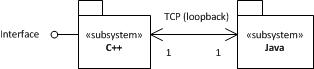
\includegraphics{figuras/arquitetura.jpg}
\caption{Visão geral da arquitetura do sistema}
\label{arquiteturaGeral}
\end{figure}


\subsection{Subsistema: Java}

A figura \ref{arquiteturaJava} apresenta a arquitetura do subsistema implementado em Java. Existem três classes principais, \emph{Manipuladora}, \emph{Comunicadora} e \emph{Level}.
A classe Manipuladora é responsável por consultar e manter atualizados os arquivos de modelos de agentes (explicados em \ref{estruturaPastas}), já a classe Comunicadora é a responsável por receber, enviar e traduzi as mensagens que chegam através da conexão com o subsitema C++. Ambas as classes se comunicam com a classe Level que nada mais é do que a classe de ambiente dos agentes. A classe Level é uma classe utilizada pelo Jason, ela representa o ambiente (enviroment) e é nela que todas as ações dos agentes foram implementadas, no caso deste programa as ações dos agentes são basicamente escolher um tipo de resposta ou atualizar variáveis de controle dos agentes e dos lugares.

\begin{figure}
\centering
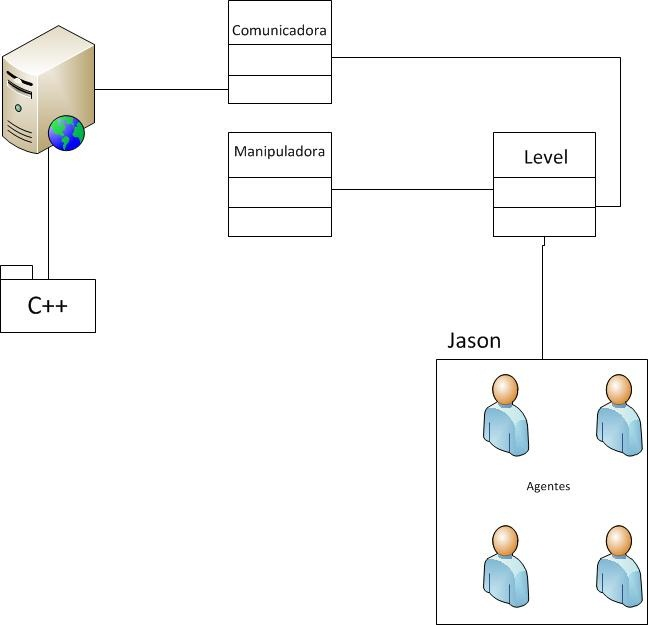
\includegraphics[width=\textwidth]{figuras/arquitetura-java.jpg}
\caption{Visão geral da arquitetura do subsistema Java}
\label{arquiteturaJava}
\end{figure}



\subsection{Subsistema: C++}



\section{Protocolo de comunicação}

A concepção do protocolo de comunicação envolveu alguns cuidados especiais, e precauóes foram tomadas no sentido de preservar a flexibilidade do protocolo --- isto é, facilitar a adição de novas mensagens no decorrer ro projeto --- e garantir certo desacoplamento entre o trabalho de modelagem de agentes e projeto do blackboard, de um lado, e a lógica do jogo, de outro. Buscou-se organizar a comunicação entre Java e C++ de modo tal que o projeto pudesse ser levado a cabo sem a necessidade de programadores de um e outro sistema precisassem saber do funcionamento do outro. Essa flexibilidade permite que as responsabilidades dos sistemas sejam alteradas durante a evolução do projeto, o que é importante para permitir a exploração de possibilidades de organização do jogo como um todo. Para isso, é necessário que os protótipos construídos não enfrentem as restrições de uma arquitetura rígida.

\section{Estrutura de pastas}\label{estruturaPastas}

O projeto foi desenvolvido com vistas a se prestar à experimentação no
design. Assim, algumas ferramentas para a escrita de \emph{scripts} de
diálogos ou pequenas cenas foram desenvolvidas.

Descrevemos a seguir a organização dos arquivos do projeto. É
importante que essa estrutura seja clara e intuitiva, já que é nossa
intenção que alguns desses arquivos (que configuram o comportamento
do jogo) sejam alterados primariamente por designers do jogo. Assim, é
preciso que haja critério na complexidade que se expõe a esses
``usuários''. A figura~\ref{fig:estrut-arquiv} exibe a distribuição de arquivos nas pastas do projeto.  

\begin{figure}
\centering
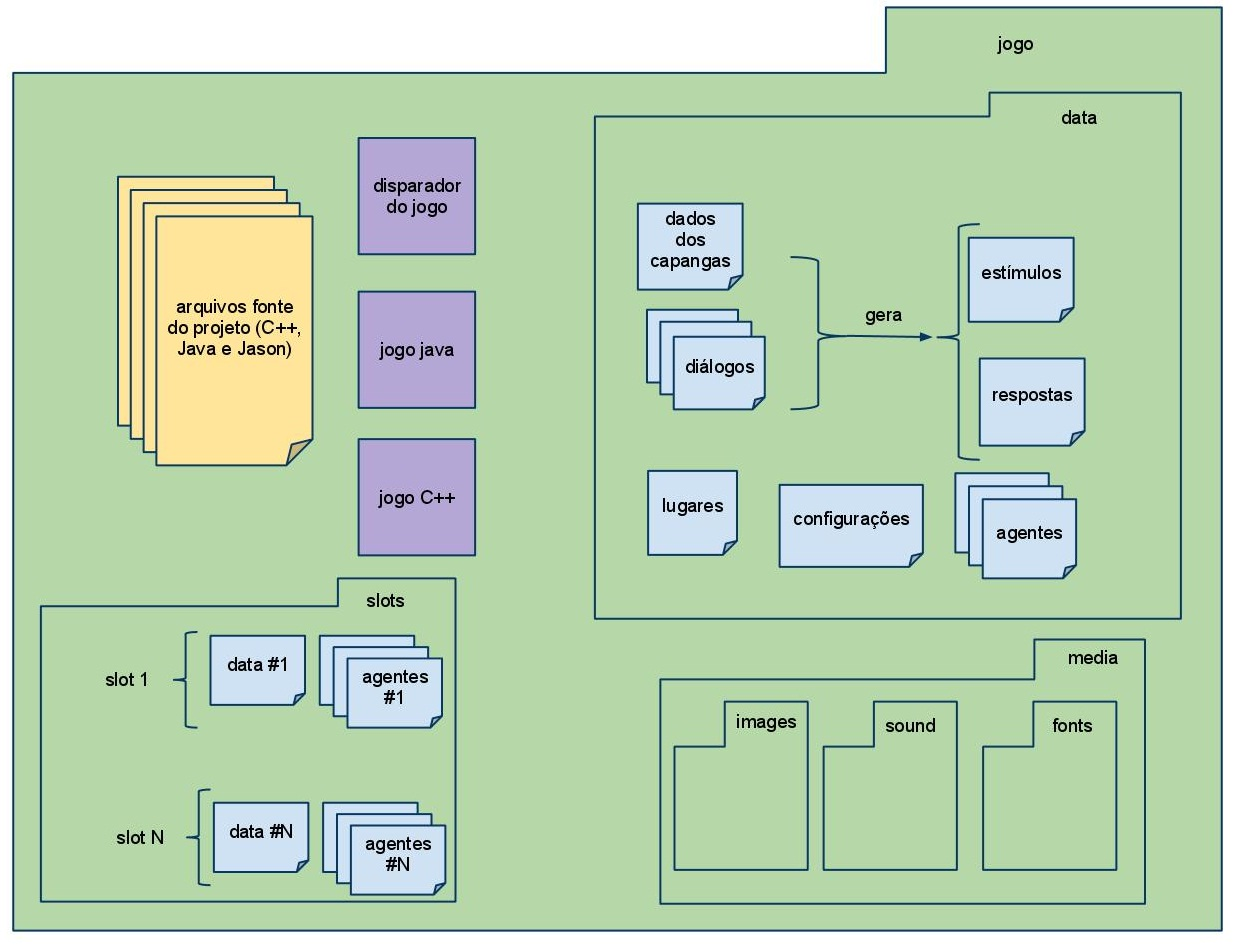
\includegraphics[width=\textwidth]{figuras/estrutura-arquivos.jpg}
\caption{Organização de arquivos do projeto}
\label{fig:estrut-arquiv}
\end{figure}


\section{Arquivos auxiliares}

Uma série de arquivos de texto auxiliares são usados pelo
jogo. São em sua maioria estáticos, e sendo que alguns são lidos por ambos os programas. Ressalta-se que os conjuntos de arquivos gerados por Java e C++ não têm intersecção, o que elimina a necessidade de gerência de situações de escrita concorrente. Eles especificam
\begin{itemize}
\item diálogos,
\item modelos de agentes,
\item informações de instâncias de agentes,
\item tipos de reações,
\item tipos de estímulos a agentes,
\item lugares passíveis de assalto,
\item dados de capangas,
\item ações da polícia.
\end{itemize}

Explicamos a seguir a função de cada um dos tipos de arquivo.

Os \emph{diálogos} são scripts que codificam possíveis dizeres que
\npc{}s ou o jogador podem efetuar em um diálogo. Carregam informação sobre
o sentimento que expressam ou a impressão que causam. Seguem a
gramática descrita no apêndice~\ref{ap:gram-script-dialogo}.

Os \emph{modelos de agentes} são arquivos de texto para controle das informações de cada agente. Possuem as seguintes informações sobre os agentes:
\begin{itemize}
\item tipo do agente: inteiro que define o tipo do agente (0-capanga,1-civil,2-policial,3-oculto).
\item id do agente: inteiro único, entre 10 e 99 que representa o agente.
\item nome do agente: String com o nome do agente.
\item personalidade: String que define a personalidade atual do agente.
\item estado psicologico: String que define o estado psicológico atual do agente.
\end{itemize}
Os itens listados acima são comuns a todos os tipos de agentes.
Além dos itens listados acima, os arquivos de agentes policiais possuem uma informação extra sobre a variável \emph{conduta} associada a cada policial, que é uma String que pode assumir dois valores (ganancioso ou íntegro), e os arquivos de agentes capangas possui a variável \emph{nível de suspeita} que é um inteiro (o valor máximo desta variável é definido no arquivo de configuração), ela serve para a polícia monitorar os capangas e decidir se deve ou não prendê-lo.
Vale citar que existe um arquivo por agente e que o nome do arquivo é sempre formado pela seguinte regra: \verb!a! + \verb!tipo-do-agente! + \verb!id-do-agente.txt!

Os \emph{tipos de estímulos, tipos de reações, lugares passíveis de assalto, dados de capangas,} e \emph{ações da polícia} são arquivos de interface, lidos por ambos os programas na decodificação de mensagens trocadas. Optou-se por essa solução para que a comunicação se desse pelo envio de inteiros, indicando qual a linha do arquivo de interface
em que a mensagem está contida. Com isso o processo de alteração do protocolo em seus estágios iniciais de desenvolvimento foi simplificado, uma vez que sua própria especificação atua como um tipo de documentação; além disso, a mudança das mensagens do protocolo passou a ser feita pela mudança de algumas linhas em um arquivo de configuração e em um mapa de strings a funções, o que facilitou a experimentação. Claramente, essa abordagem só é
possível porque as mensagens são conhecidas \emph{a priori}.

Para comunicar o estímulo que uma determinada fala no diálogo provoca
no agente, a lógica do jogo envia ao sistema BDI um inteiro indicando
a linha em que está escrita a string que define o estado. Na prática,
a lógica do jogo faz uma chamada para enviar o inteiro correspondente
ao estímulo que se deseja comunicar, e uma busca é feita no arquivo
que contém os estímulos possíveis para encontrar o conteúdo da linha
correspondente. Essa string é, por fim, enviada ao sistema BDI, que
fará a sua própria busca para identificar qual o estímulo recebido.

Vale notar que os arquivos contendo os estímulos e reações são gerados por um programa que os extrai dos diálogos escritos para o jogo.


